% This file was created with tikzplotlib v0.10.1.
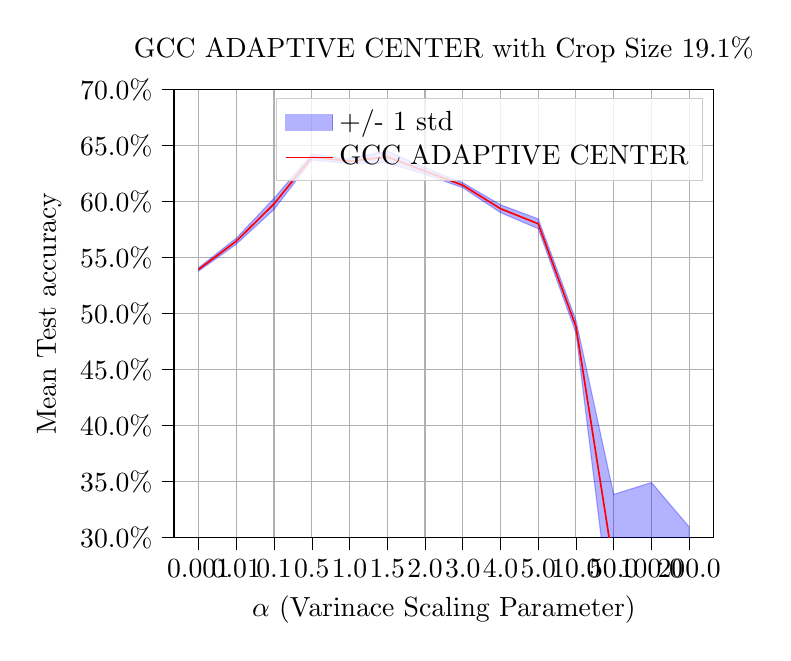
\begin{tikzpicture}

\definecolor{darkgray176}{RGB}{176,176,176}
\definecolor{lightgray204}{RGB}{204,204,204}

\begin{axis}[
legend cell align={left},
legend style={fill opacity=0.8, draw opacity=1, text opacity=1, draw=lightgray204},
tick align=outside,
tick pos=left,
title={GCC ADAPTIVE CENTER with Crop Size 19.1\%},
x grid style={darkgray176},
xlabel={\(\displaystyle \alpha\) (Varinace Scaling Parameter)},
xmajorgrids,
xmin=-0.65, xmax=13.65,
xtick style={color=black},
xtick={0,1,2,3,4,5,6,7,8,9,10,11,12,13},
xtick={0,1,2,3,4,5,6,7,8,9,10,11,12,13},
xticklabels={0.001,0.01,0.1,0.5,1.0,1.5,2.0,3.0,4.0,5.0,10.0,50.0,100.0,200.0},
xticklabels={0.001,0.01,0.1,0.5,1.0,1.5,2.0,3.0,4.0,5.0,10.0,50.0,100.0,200.0},
y grid style={darkgray176},
ylabel={Mean Test accuracy},
ymajorgrids,
ymin=0.3, ymax=0.7,
ytick style={color=black},
ytick={0.3,0.35,0.4,0.45,0.5,0.55,0.6,0.65,0.7},
yticklabels={30.0\%,35.0\%,40.0\%,45.0\%,50.0\%,55.0\%,60.0\%,65.0\%,70.0\%}
]
\path [draw=blue, fill=blue, opacity=0.3]
(axis cs:0,0.540929705854078)
--(axis cs:0,0.537870294145922)
--(axis cs:1,0.561912994231491)
--(axis cs:2,0.592916253518613)
--(axis cs:3,0.636937920612253)
--(axis cs:4,0.633867708587771)
--(axis cs:5,0.634477093525776)
--(axis cs:6,0.624253209788096)
--(axis cs:7,0.612330499297486)
--(axis cs:8,0.590111925077257)
--(axis cs:9,0.575734574811783)
--(axis cs:10,0.482829540531228)
--(axis cs:11,0.209839060799996)
--(axis cs:12,0.230994301486106)
--(axis cs:13,0.284646800409495)
--(axis cs:13,0.309653199590505)
--(axis cs:13,0.309653199590505)
--(axis cs:12,0.349305698513894)
--(axis cs:11,0.338610939200004)
--(axis cs:10,0.494020459468772)
--(axis cs:9,0.584515425188217)
--(axis cs:8,0.597088074922743)
--(axis cs:7,0.616719500702514)
--(axis cs:6,0.629896790211904)
--(axis cs:5,0.645122906474224)
--(axis cs:4,0.638132291412229)
--(axis cs:3,0.642262079387747)
--(axis cs:2,0.602833746481387)
--(axis cs:1,0.567287005768509)
--(axis cs:0,0.540929705854078)
--cycle;
\addlegendimage{area legend, draw=blue, fill=blue, opacity=0.3}
\addlegendentry{+/- 1 std}

\addplot [semithick, red, opacity=1]
table {%
0 0.5394
1 0.5646
2 0.597875
3 0.6396
4 0.636
5 0.6398
6 0.627075
7 0.614525
8 0.5936
9 0.580125
10 0.488425
11 0.274225
12 0.29015
13 0.29715
};
\addlegendentry{GCC ADAPTIVE CENTER}
\end{axis}

\end{tikzpicture}
